\chapter{Search for MSSM $\PH \to hh \to \Pgt\Pgt bb$}
\label{chap:Hhh}

As described in detail in section~\ref{chap:theory}, there are many popular MSSM
models which incorporate the 125 GeV Higgs. As seen in Chapter
\ref{chap:httmssm}, the $\PH \to \Pgt\Pgt$ analysis is very successful in 
setting limits on various MSSM models. The $\PH \to \Pgt \Pgt$ result primarily sets
limits on the high $\tan\beta$ regions, and so with large amounts of the
$m_{A}-\tan\beta$plane ruled out for such MSSM scenarios, focus shifts more 
to the regions which are still allowed, in particular the low $\tan\beta$.

In certain low $\tan\beta$ regions of the MSSM, the branching ratio for the
decay of the heavy neutral scalar Higgs, H, into two of the light Higgs bosons, h,
BR($\PH \to hh$), is enhanced. Thus we could consider models in which the
light Higgs has a mass of 125 GeV and is the Higgs particle discovered at the
LHC, and as such we could get production of a pair of these light Higgs from the
heavier Higgs in the MSSM. The range of heavy Higgs masses in consideration is from 260 GeV
(driven by the kinematic threshold for the producton of two 125 GeV Higgs
bosons) up to 350 GeV (above which the branching ratio for Higgs decaying into
tops becomes overwhelmingly high).

When looking for two 125 GeV Higgs bosons, the final state consisting of two
$\tau$ leptons and two b quarks has some sensitivity. Hence we can use the
inclusive selection from the $\PH \to \Pgt\Pgt$ and require additional jets
to form the $h \to bb$. In this way we can use a large amount of the
expertise and methods from chapters \ref{chap:httsm} and \ref{chap:httmssm}, 
to design a new analysis to target $\PH \to hh \to \Pgt\Pgt bb$.

\section{Event Selection}

\section{Control Plots}

For the preselection and separation of events into categories, there are several
kinematic variables of interest. A selection of these including b-jet related
variables, kinematics of the tau candidates, $\MET$ and $m_{T}$ are shown in
Figs.~\ref{fig:resultsControlPlotsTauPairMuTau}
and~\ref{fig:resultsControlPlotsJetPairMuTau} for the $\mu\tau_{had}$ channel
, Figs.~\ref{fig:resultsControlPlotsTauPairETau} and
~\ref{fig:resultsControlPlotsJetPairETau} for the $e\tau_{had}$ channel.
These plots are made before events are split into categories, and use all events
with all least 2 jets (no additional b-tag requirements).


\begin{figure}
\begin{center}
\subfloat[]{
    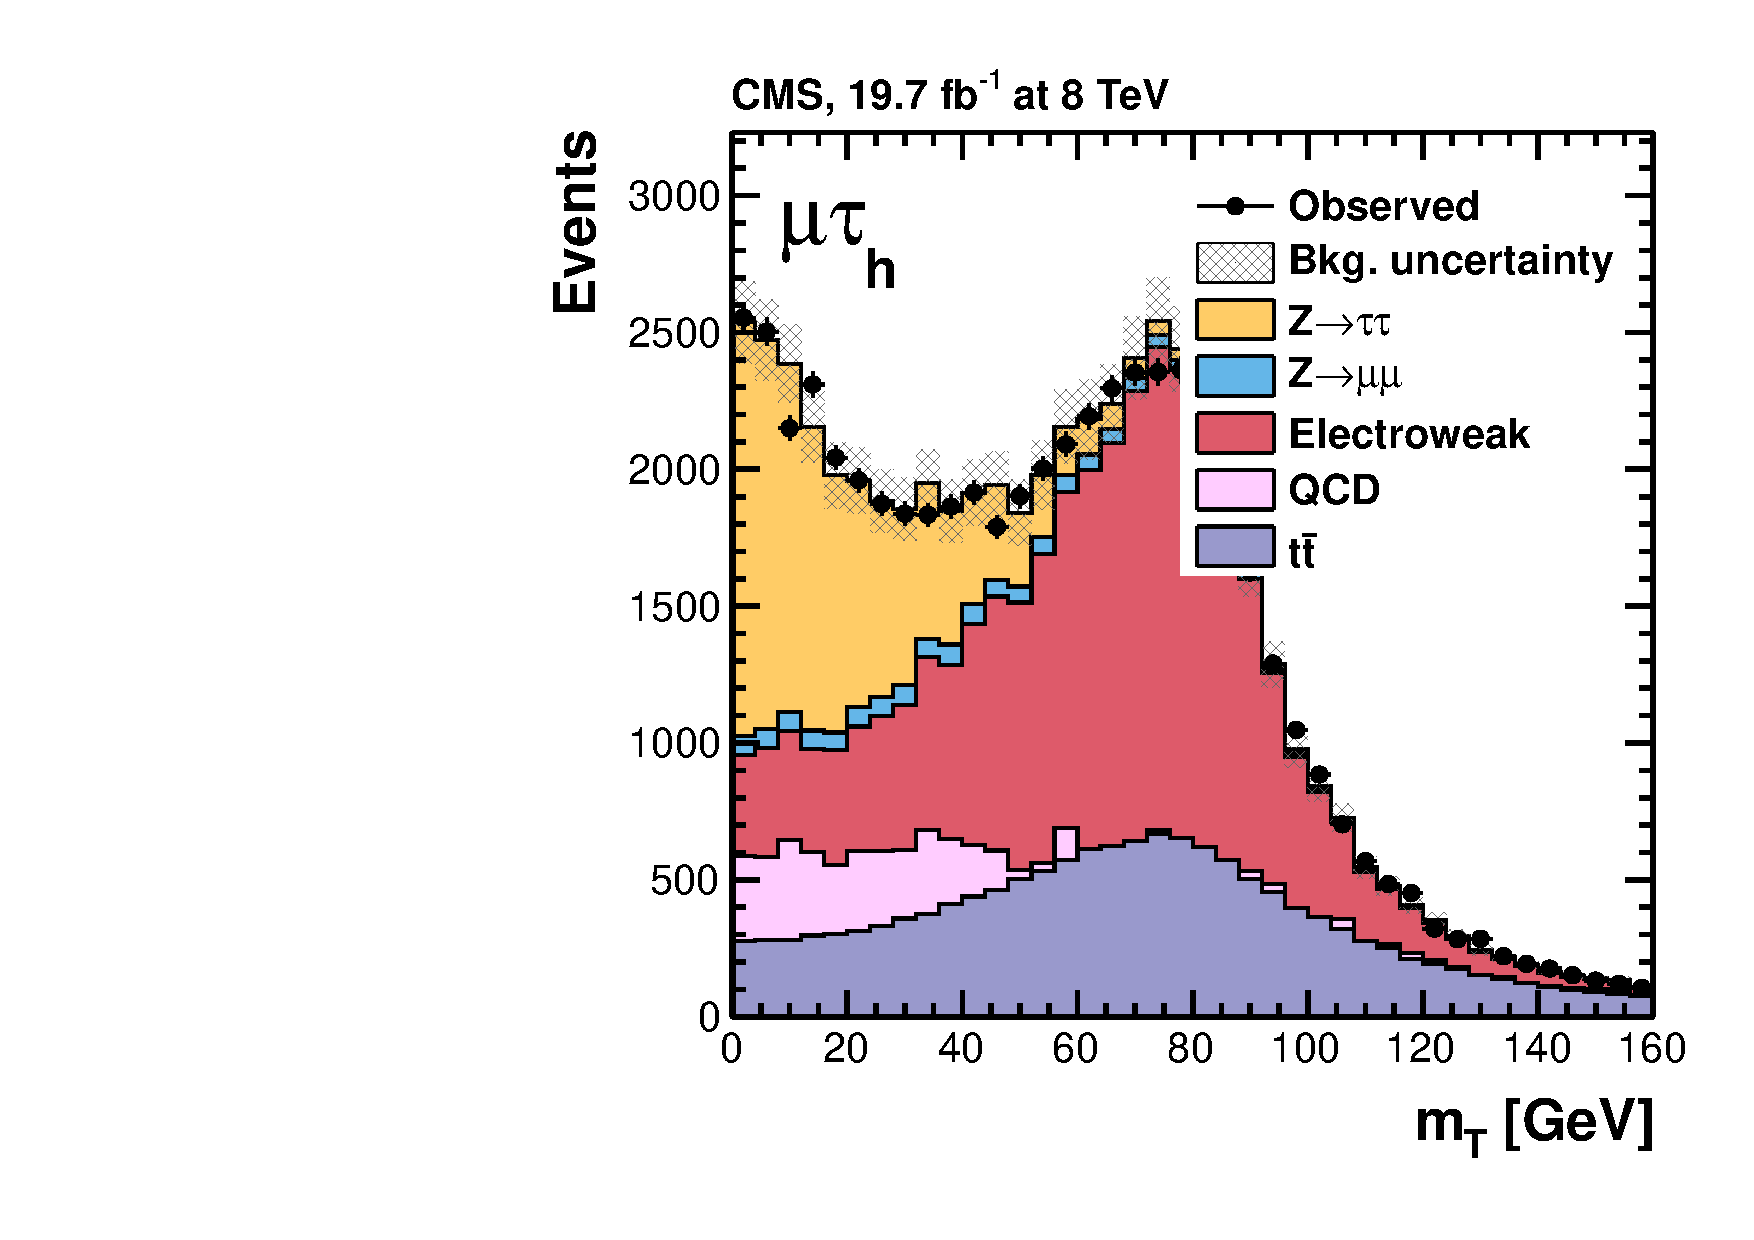
\includegraphics[width=0.4\textwidth]
      {plots/Hhh/ControlPlots/mutau/mt_1_2jetinclusive_mt_2012.pdf}}
\subfloat[]{
    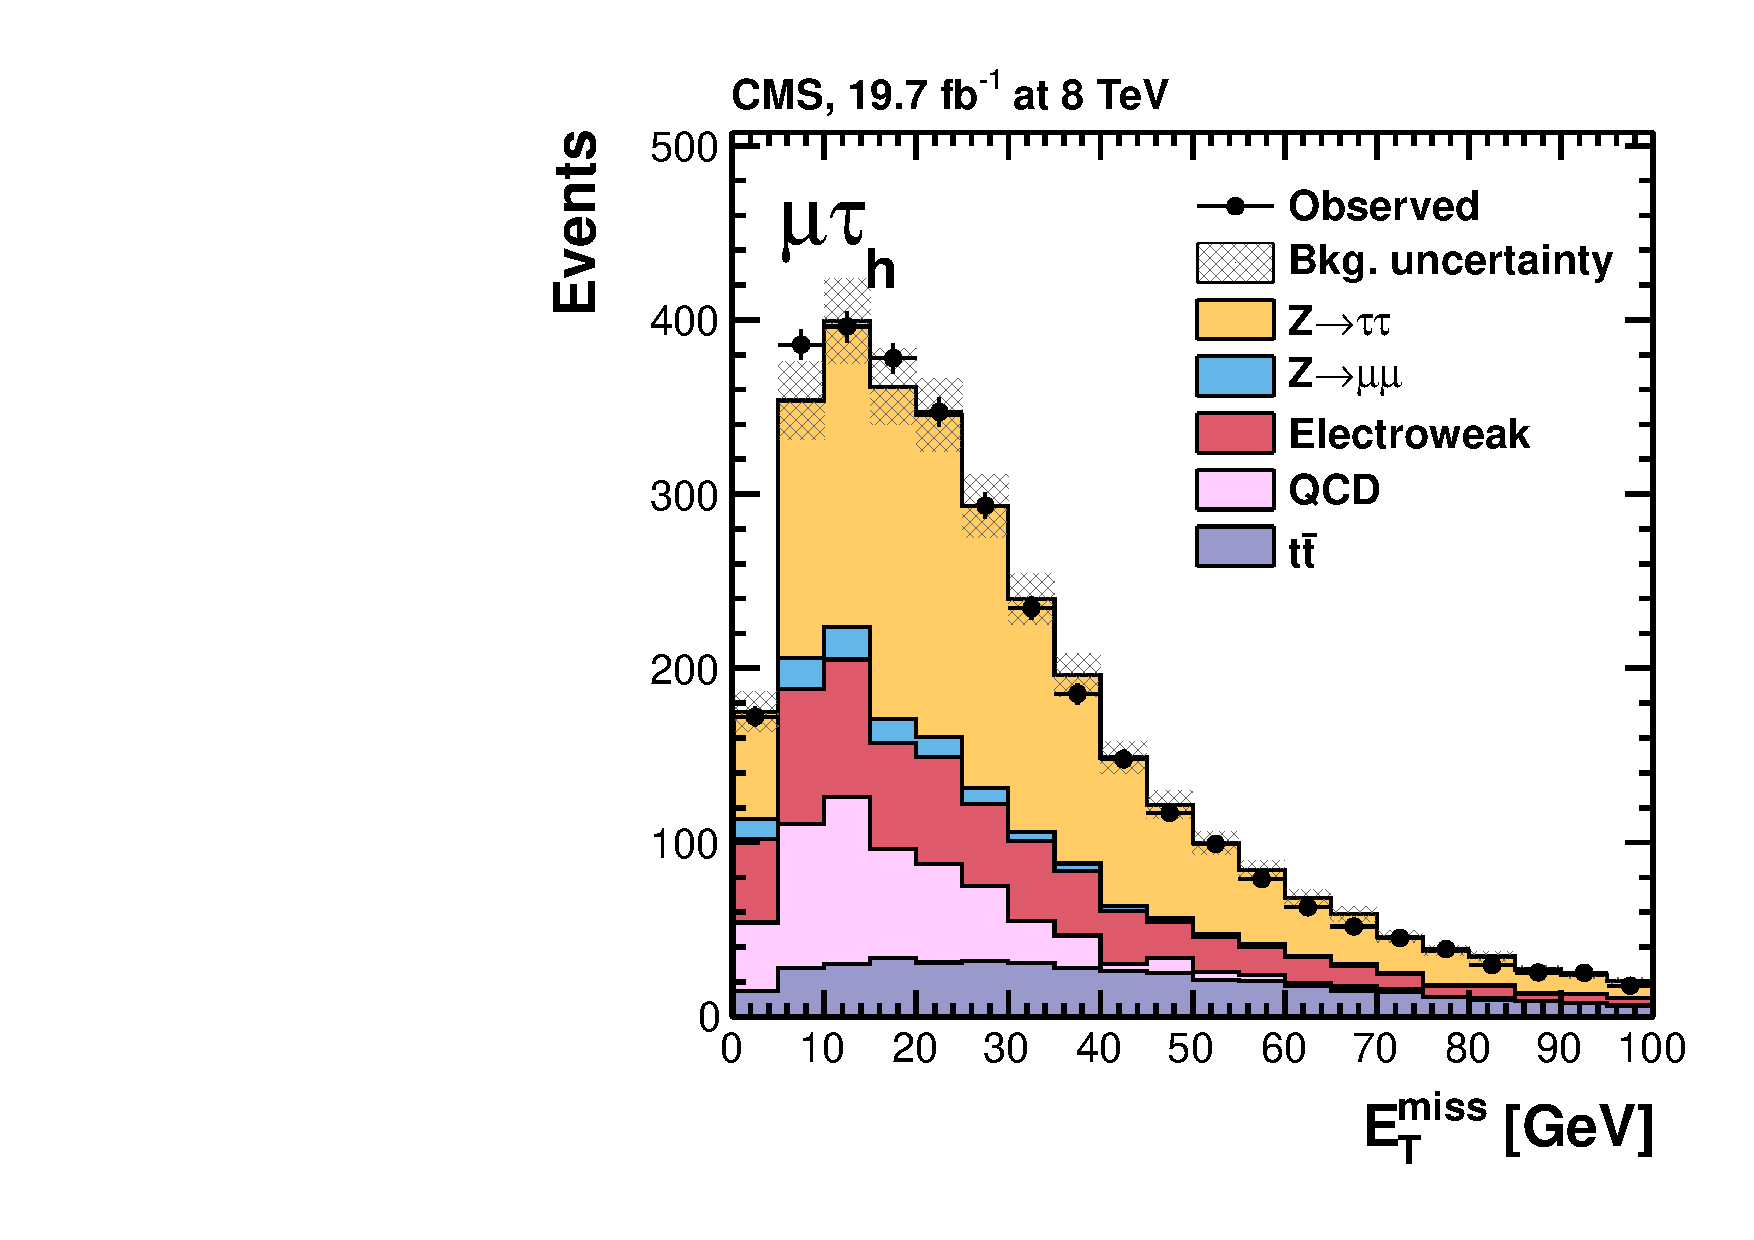
\includegraphics[width=0.4\textwidth] 
      {plots/Hhh/ControlPlots/mutau/met_2jetinclusive_mt_2012.pdf}} 

\subfloat[]{
    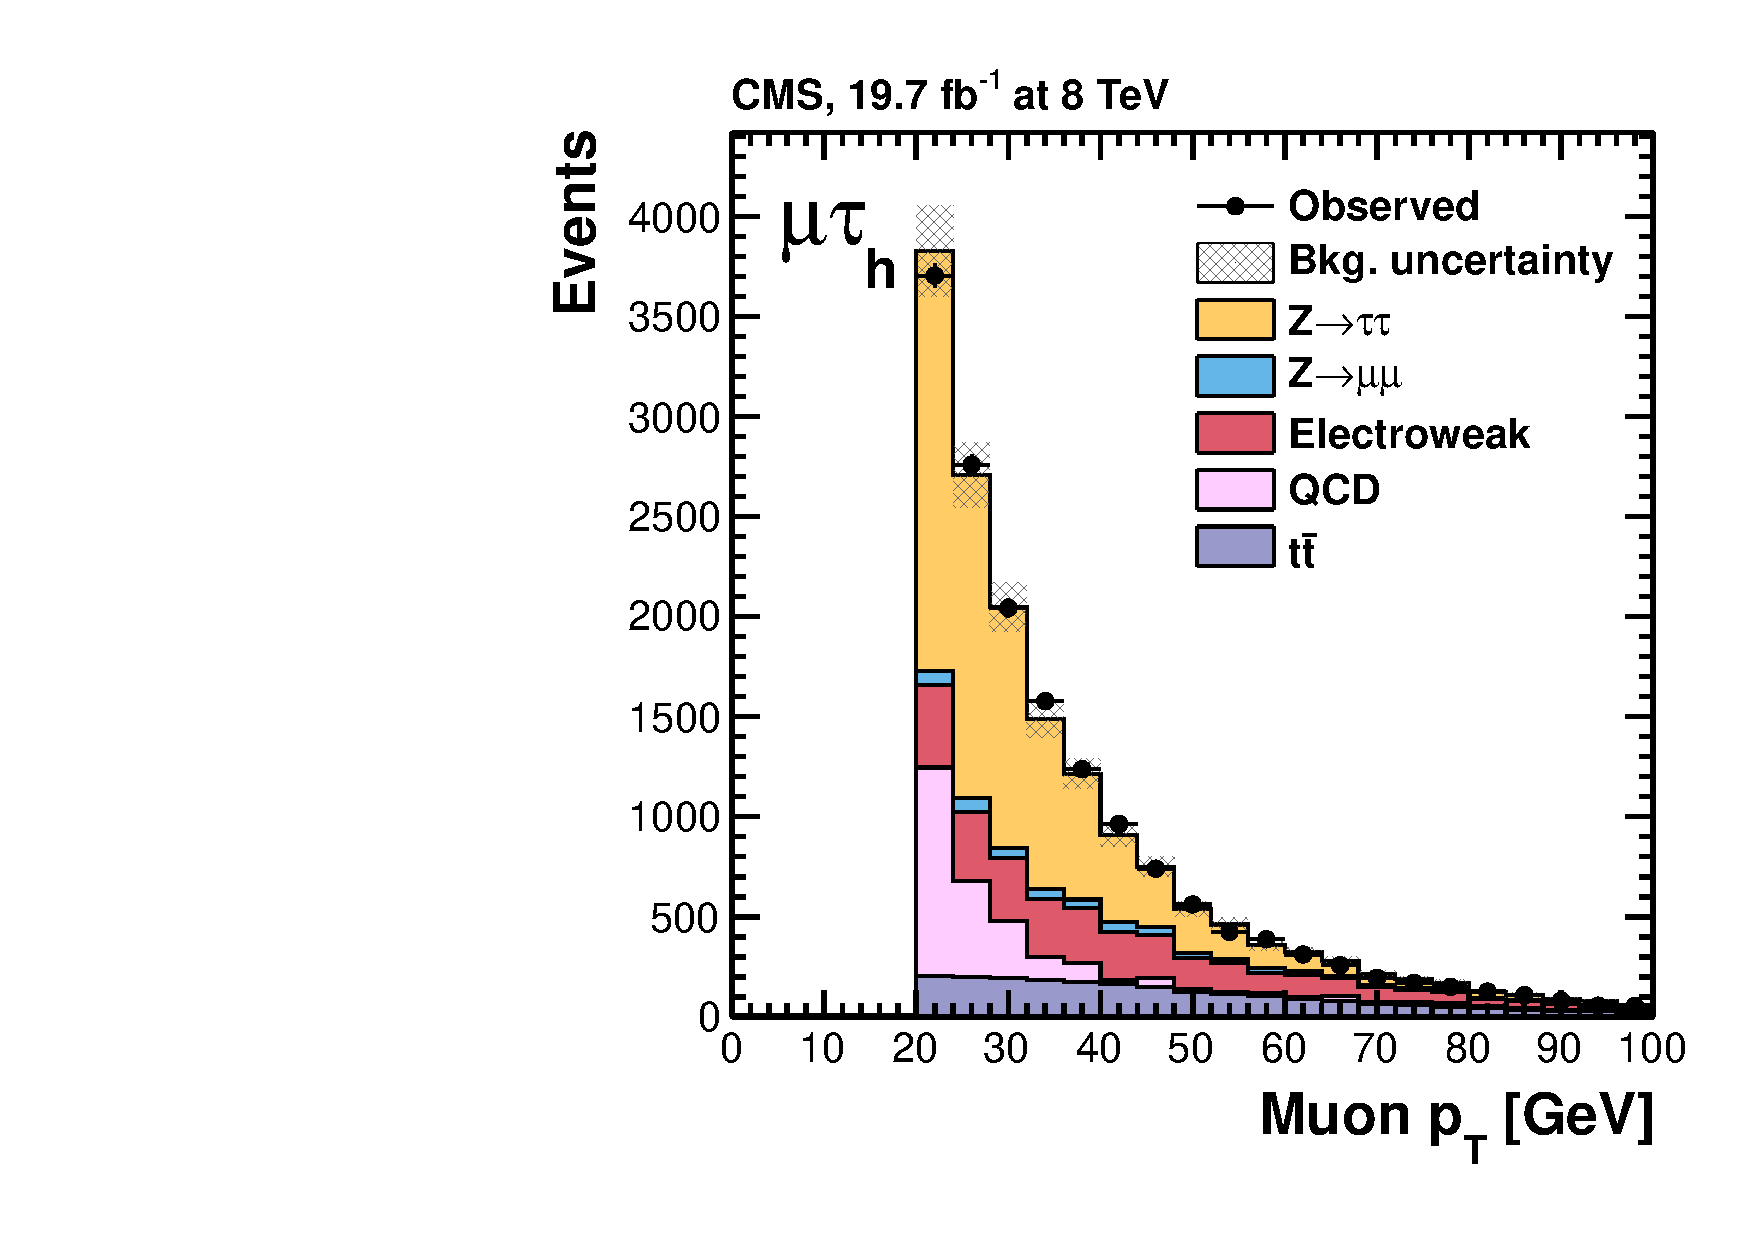
\includegraphics[width=0.4\textwidth]
      {plots/Hhh/ControlPlots/mutau/pt_1_2jetinclusive_mt_2012.pdf}}
\subfloat[]{
    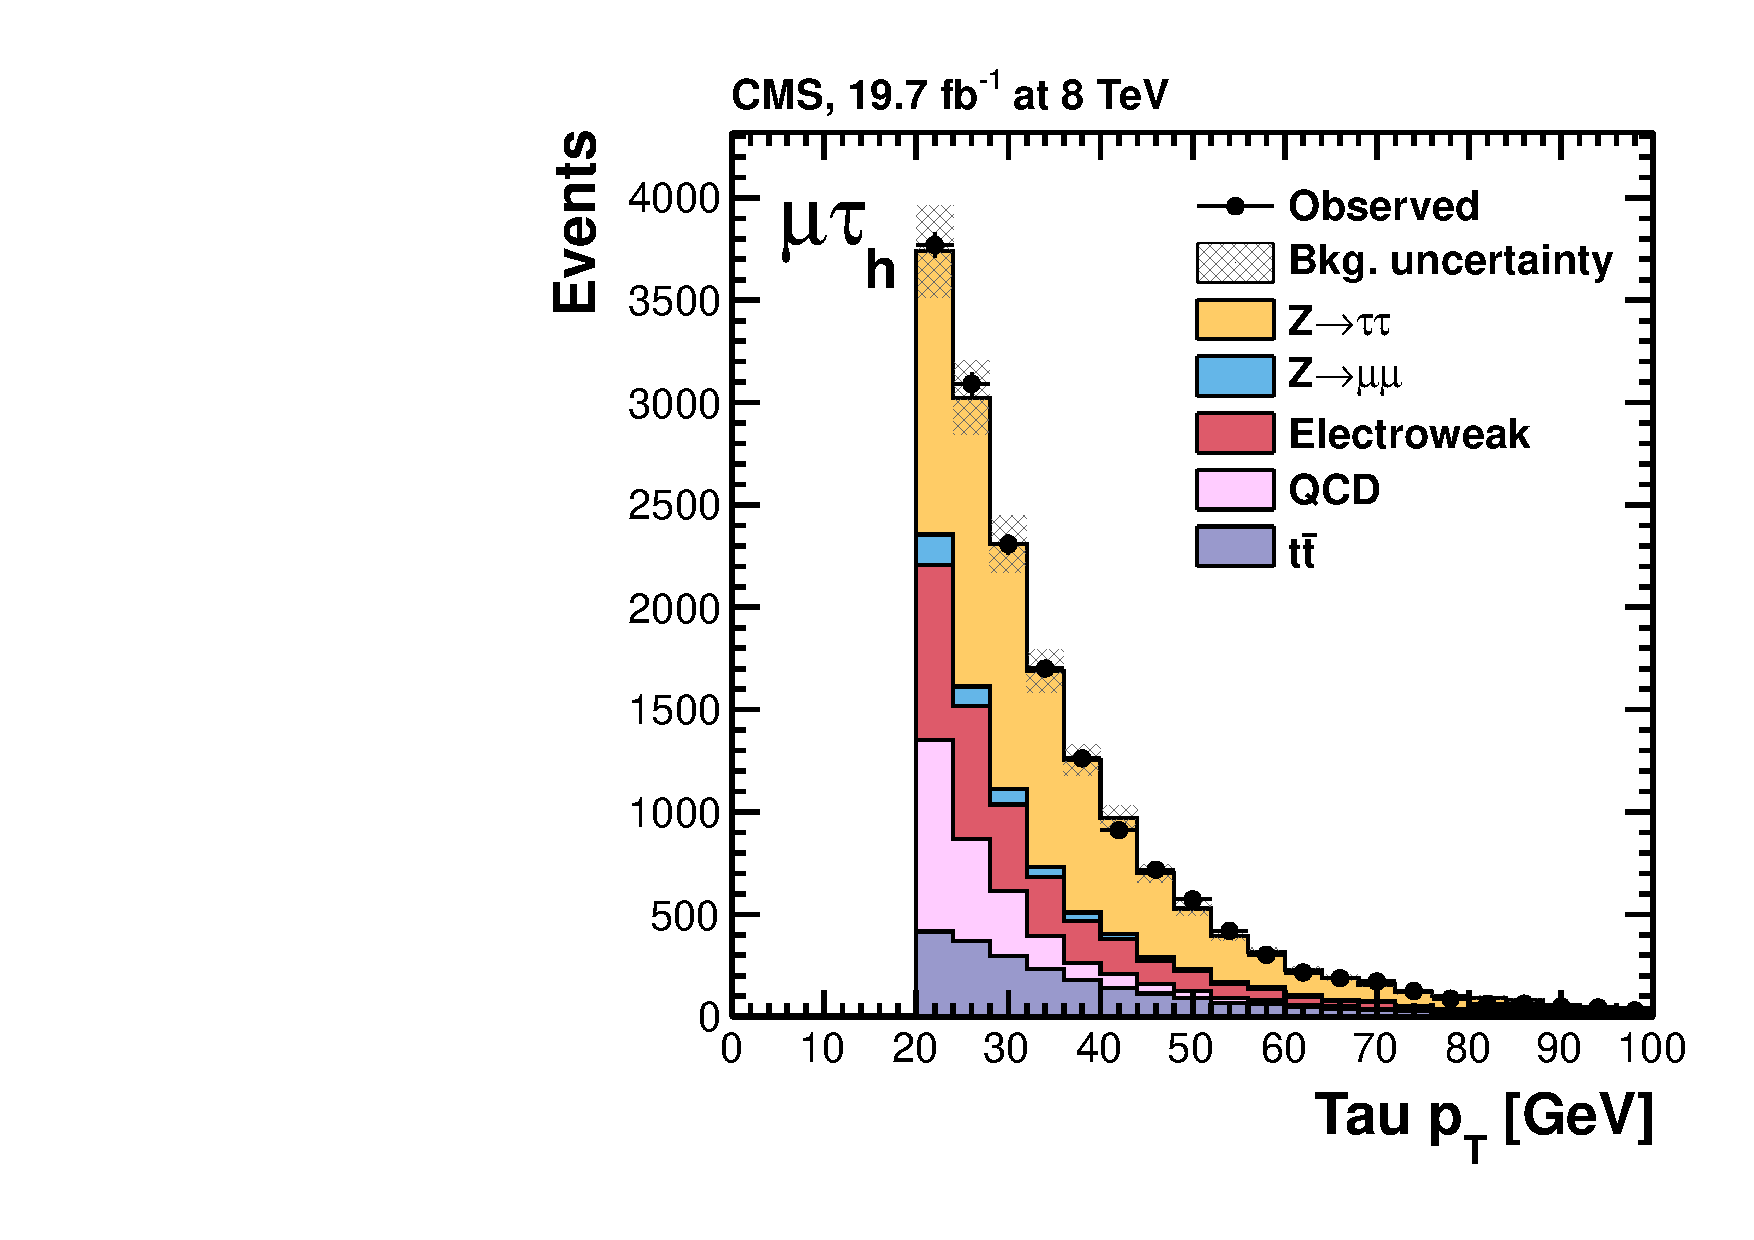
\includegraphics[width=0.4\textwidth]
      {plots/Hhh/ControlPlots/mutau/pt_2_2jetinclusive_mt_2012.pdf}} 

\subfloat[]{
    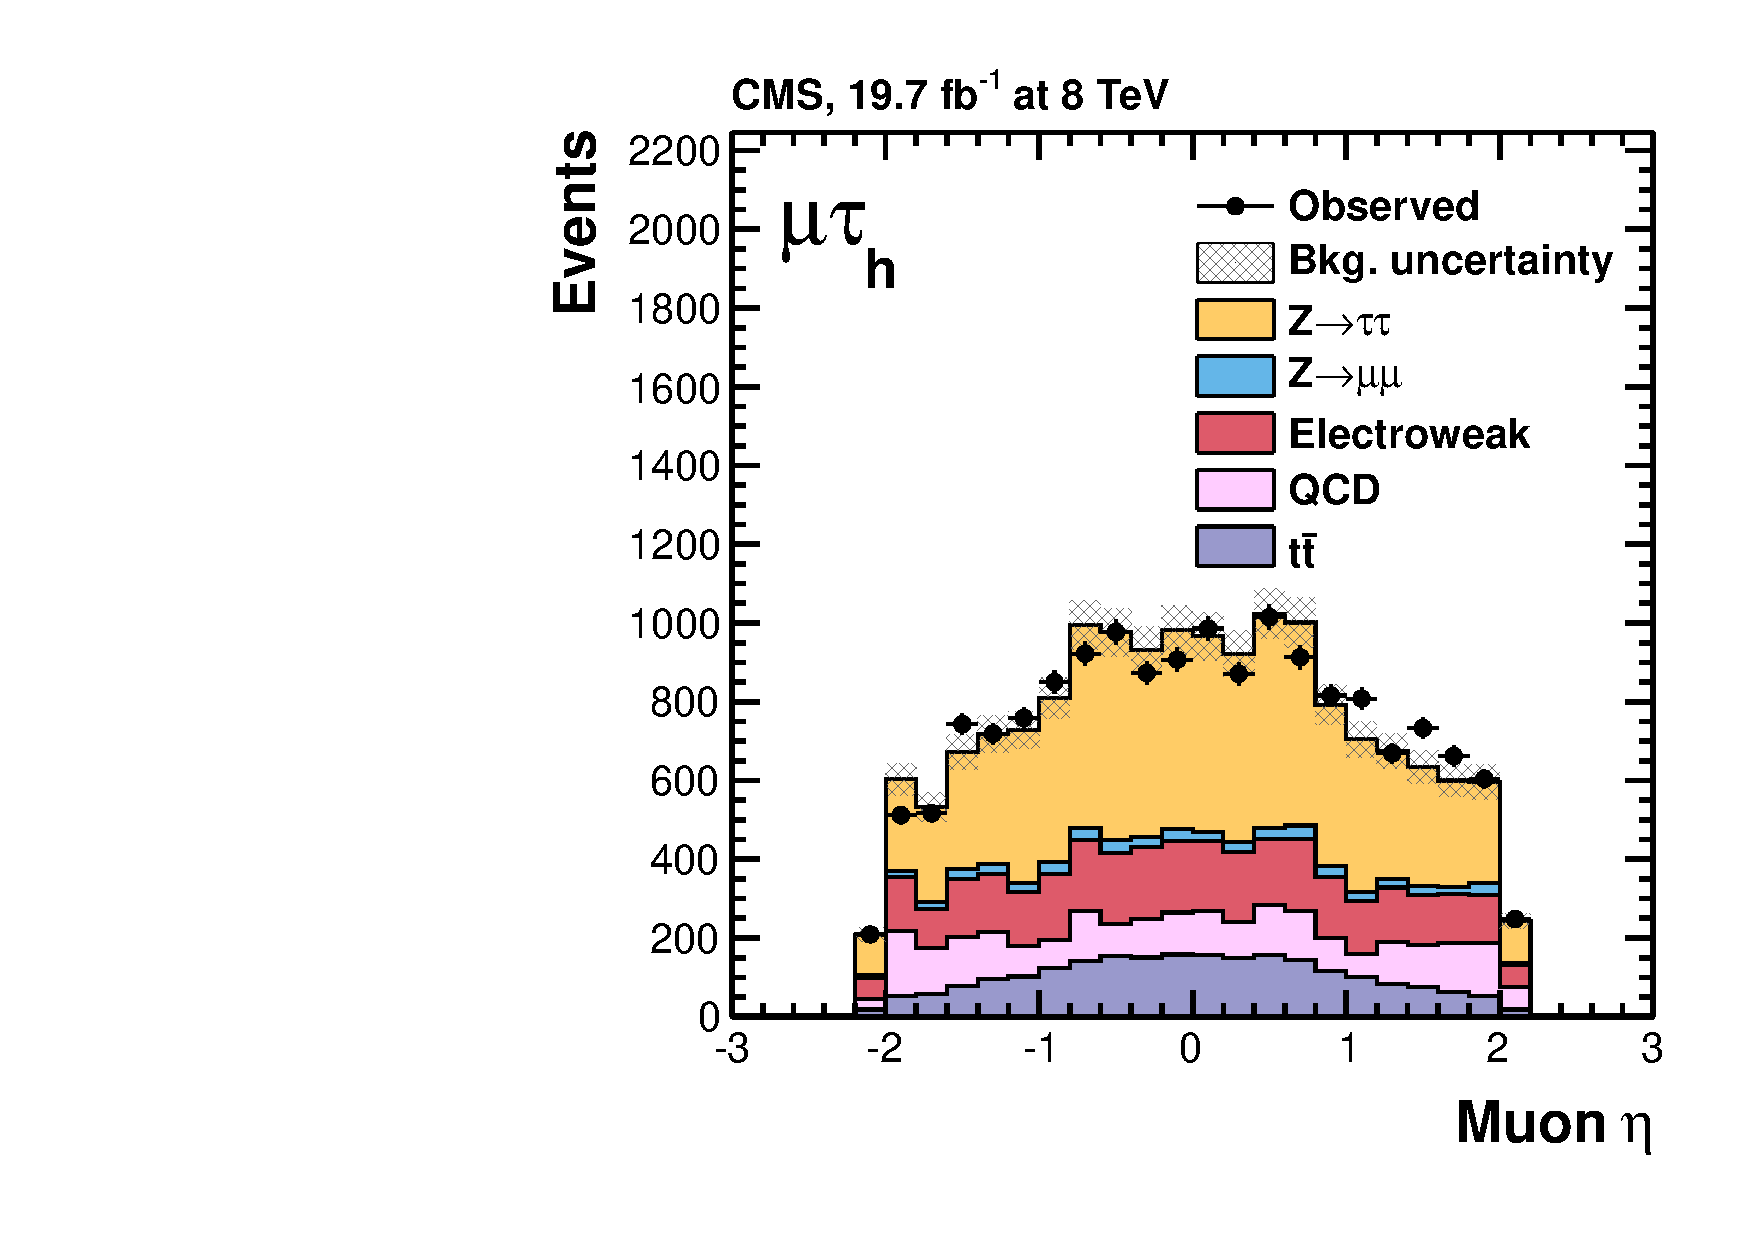
\includegraphics[width=0.4\textwidth]
      {plots/Hhh/ControlPlots/mutau/eta_1_2jetinclusive_mt_2012.pdf}}
\subfloat[]{
    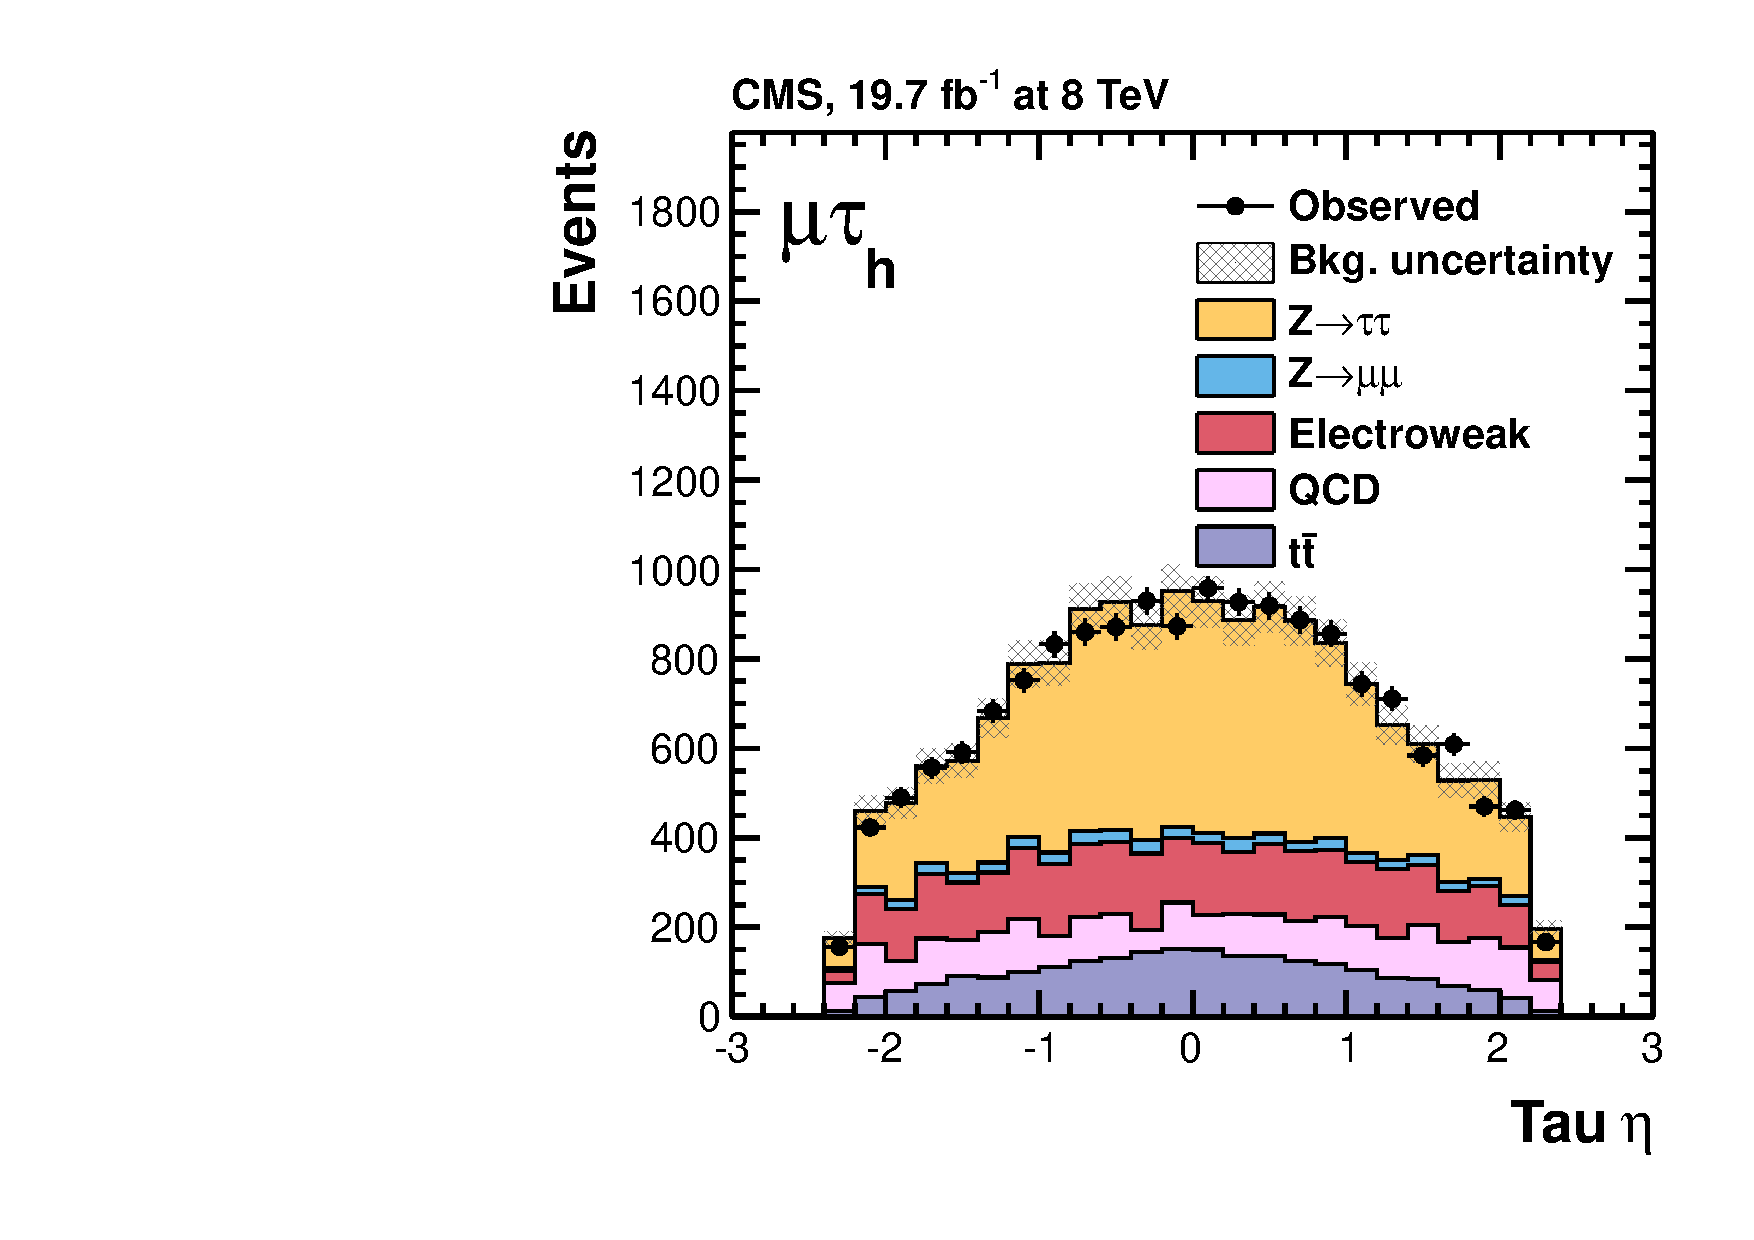
\includegraphics[width=0.4\textwidth]
      {plots/Hhh/ControlPlots/mutau/eta_2_2jetinclusive_mt_2012.pdf}}
\end{center}
\caption{
  Distributions of relevant kinematic variables for events with at least 2 jets
  in the $\mu\tau_{had}$ channel. The variable shown in a) is $m_{T}$, on which
  a cut of $m_{T} < 30$ is applied for the rest of the plots, which
  show b) $\MET$, c) $\pt$ of the muon, d) $\pt$ of the tau, e) $\eta$ of the
  muon and f) $\eta$ of the tau. 
  Expected background contributions are shown for the values of nuisance parameters
  obtained by fitting the signal plus background hypothesis to the data.
}
\label{fig:resultsControlPlotsTauPairMuTau}
\end{figure} 

\begin{figure}
\begin{center}
\subfloat[]{
    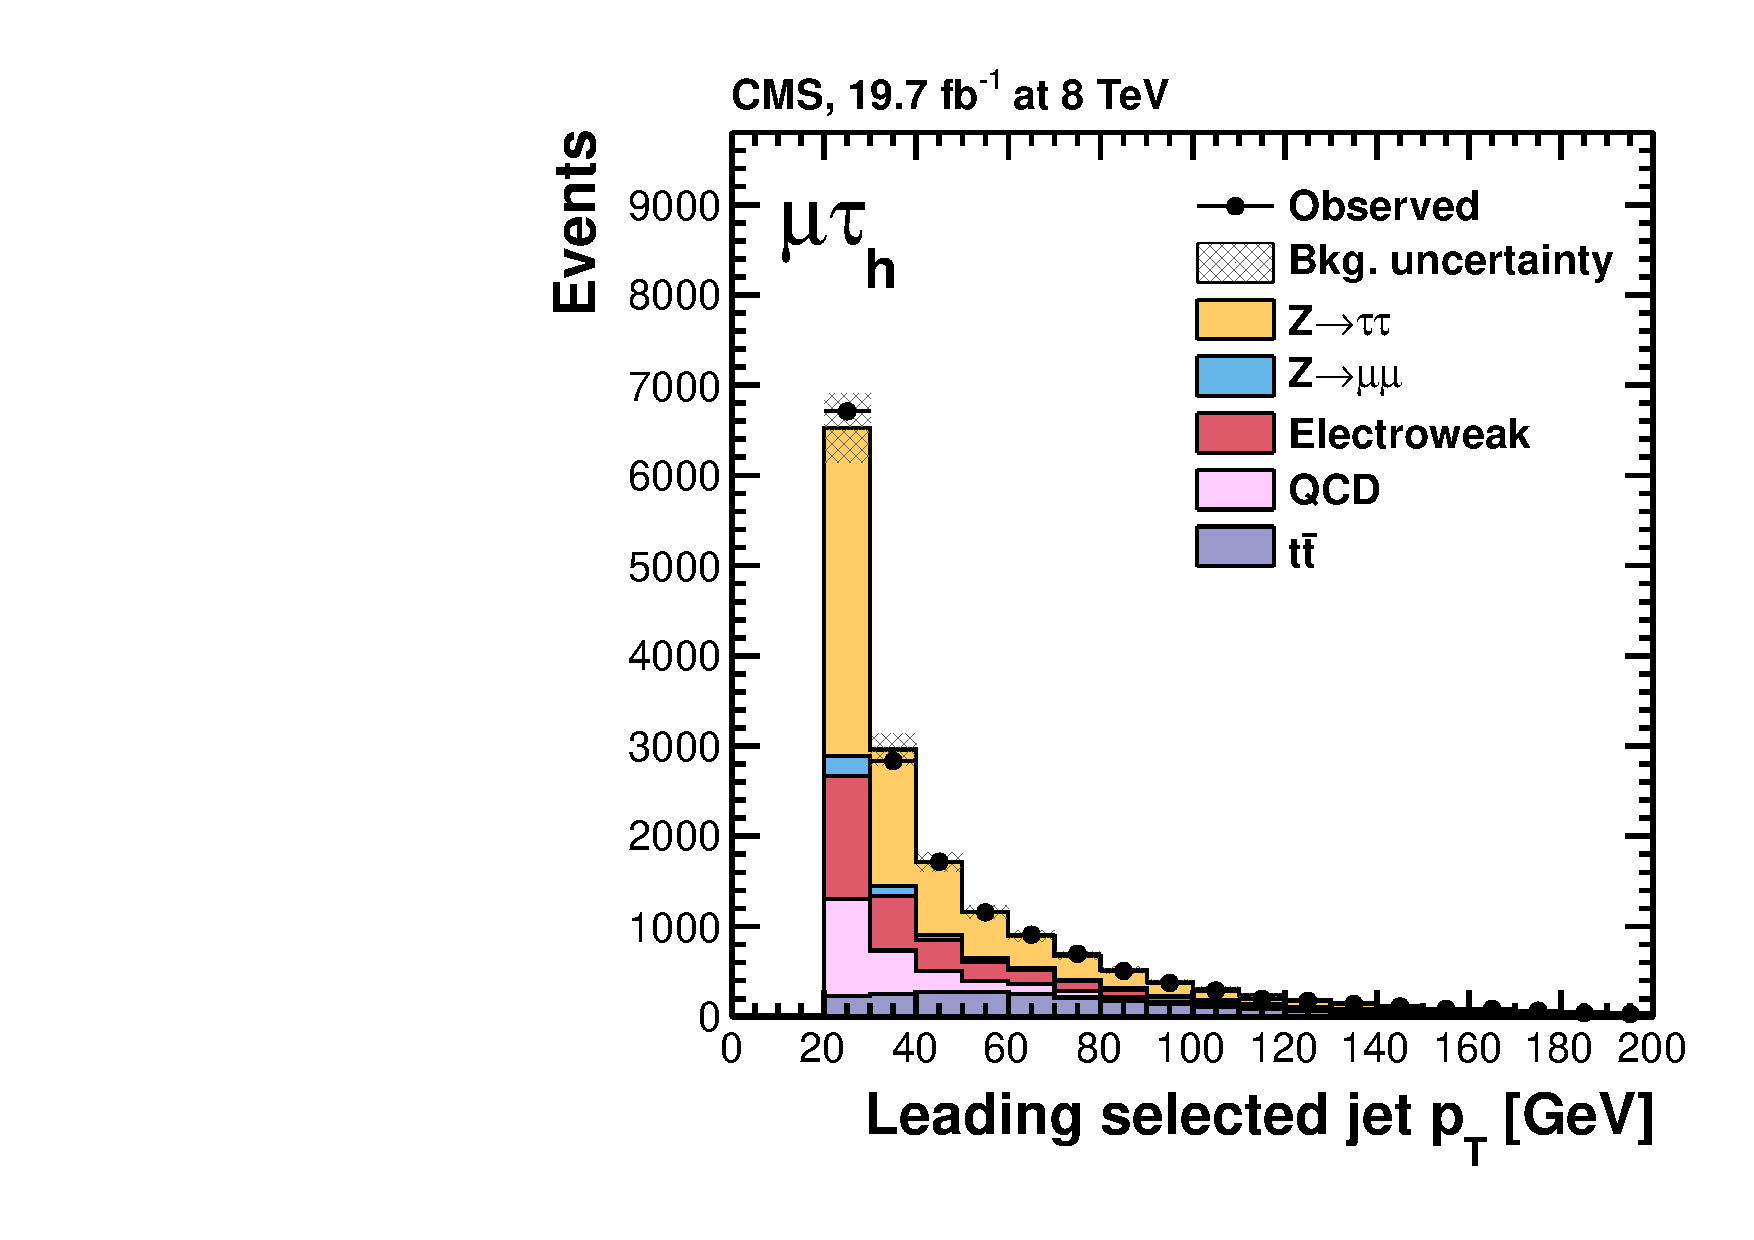
\includegraphics[width=0.4\textwidth]
      {plots/Hhh/ControlPlots/mutau/prebjetpt_1_2jetinclusive_mt_2012.pdf}}
\subfloat[]{
    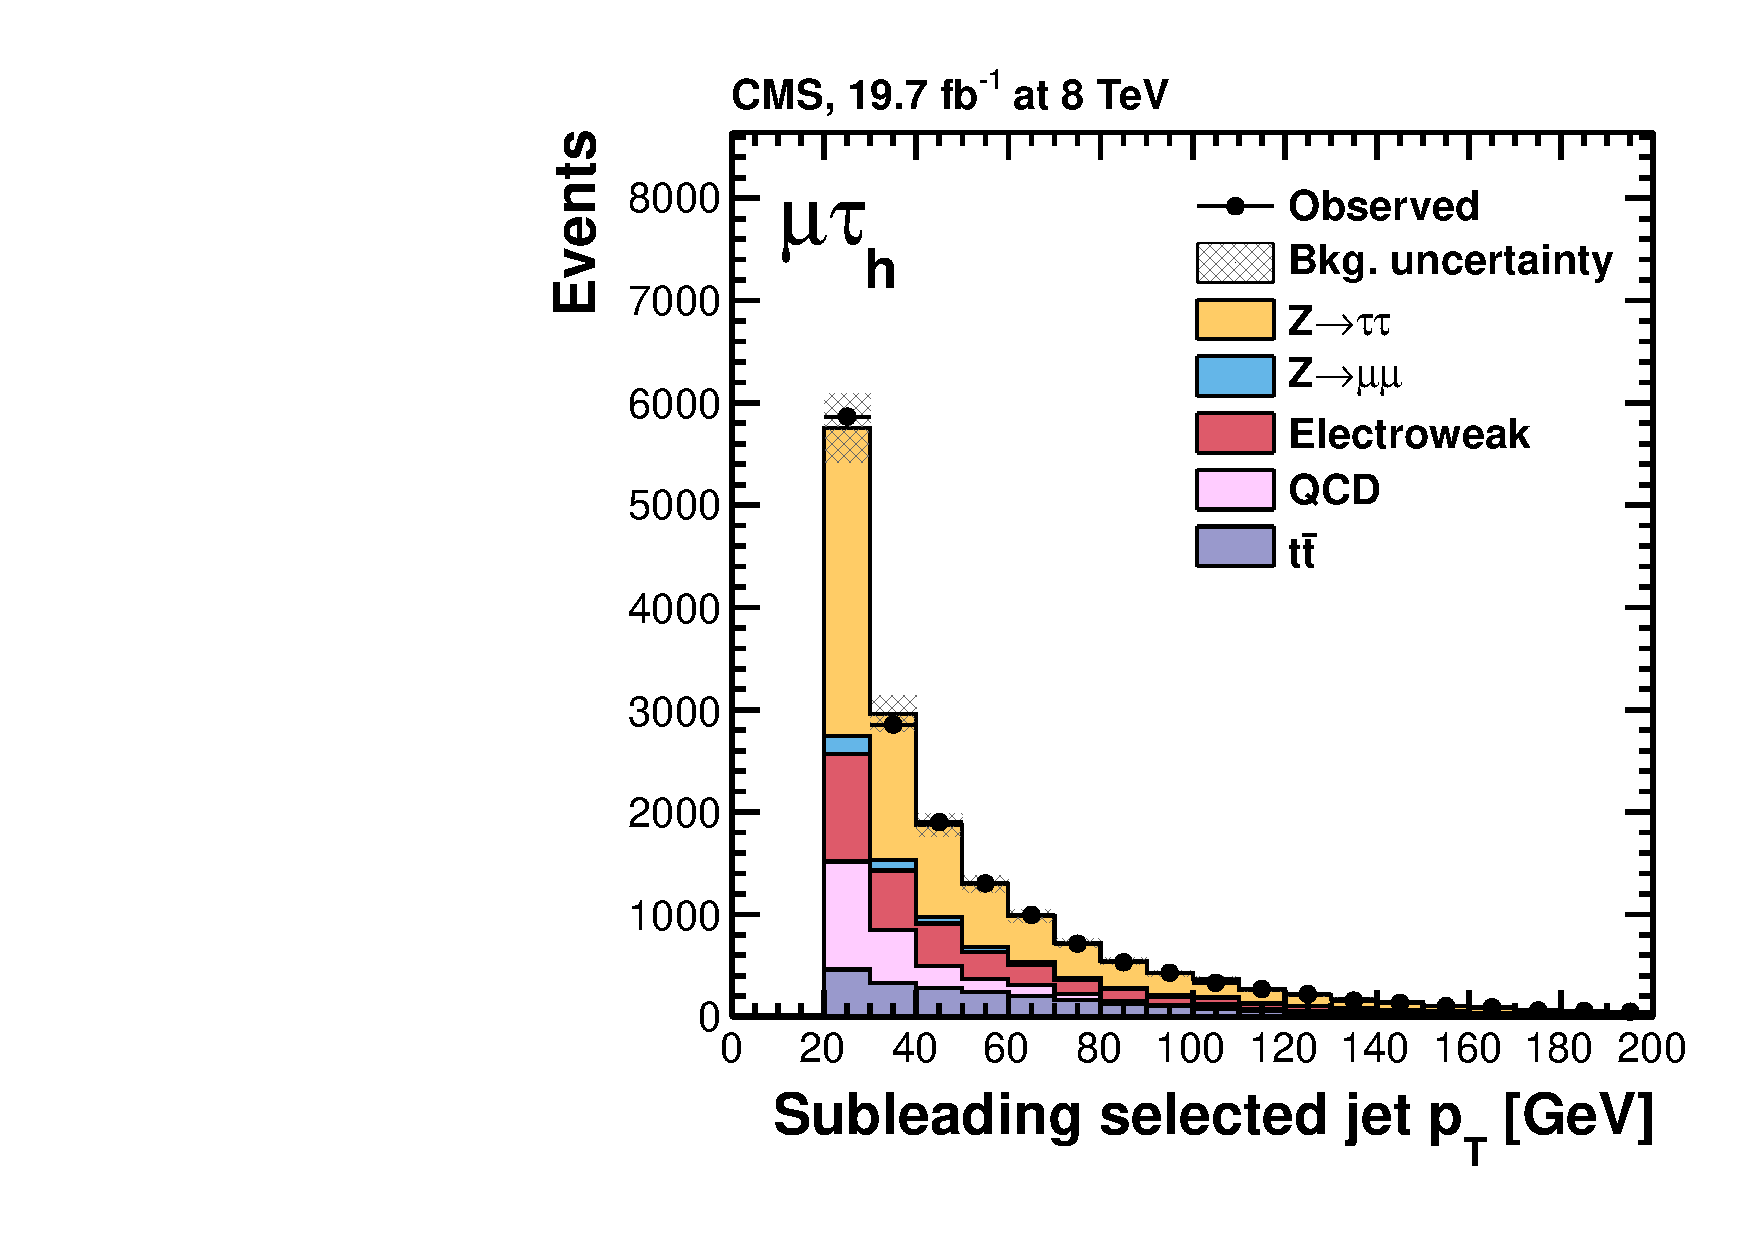
\includegraphics[width=0.4\textwidth] 
      {plots/Hhh/ControlPlots/mutau/prebjetpt_2_2jetinclusive_mt_2012.pdf}} 

\subfloat[]{
    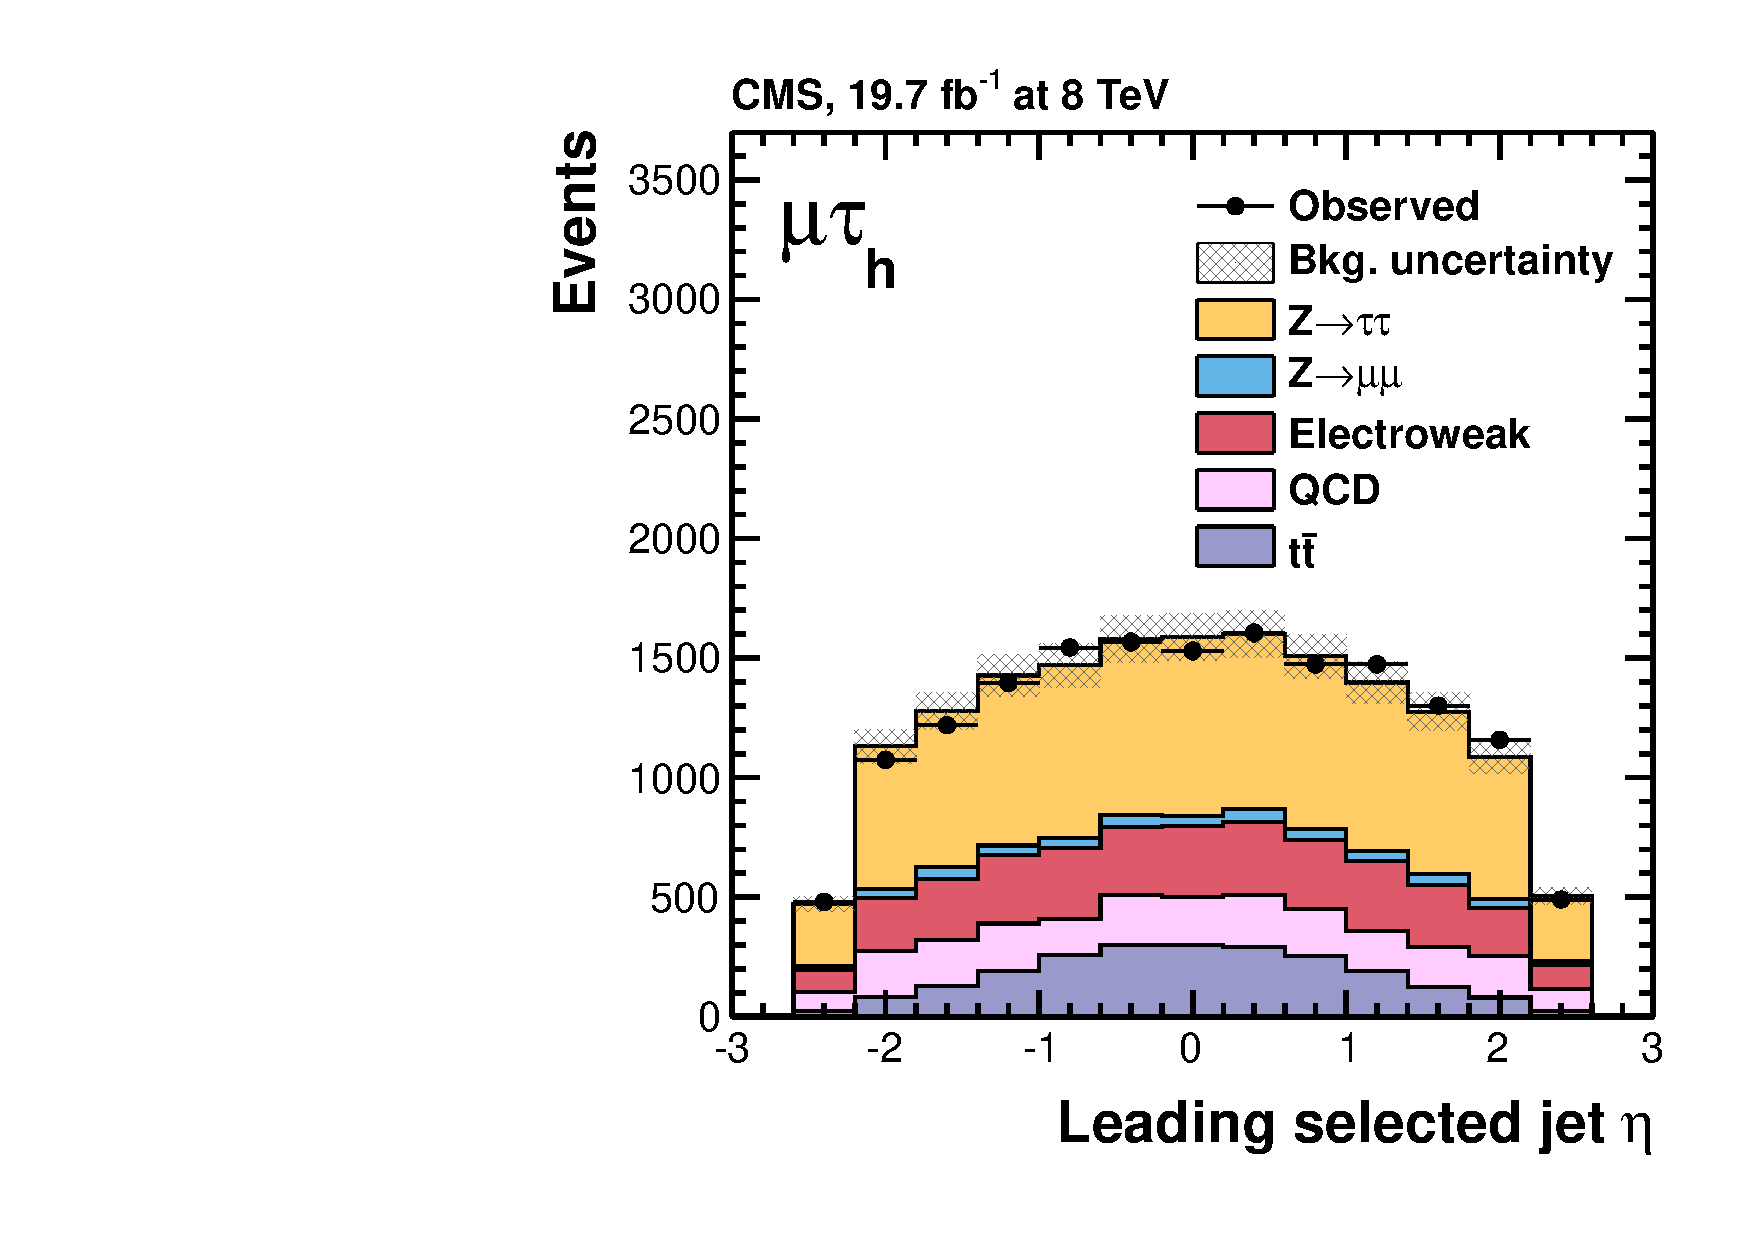
\includegraphics[width=0.4\textwidth]
      {plots/Hhh/ControlPlots/mutau/prebjeteta_1_2jetinclusive_mt_2012.pdf}}
\subfloat[]{
    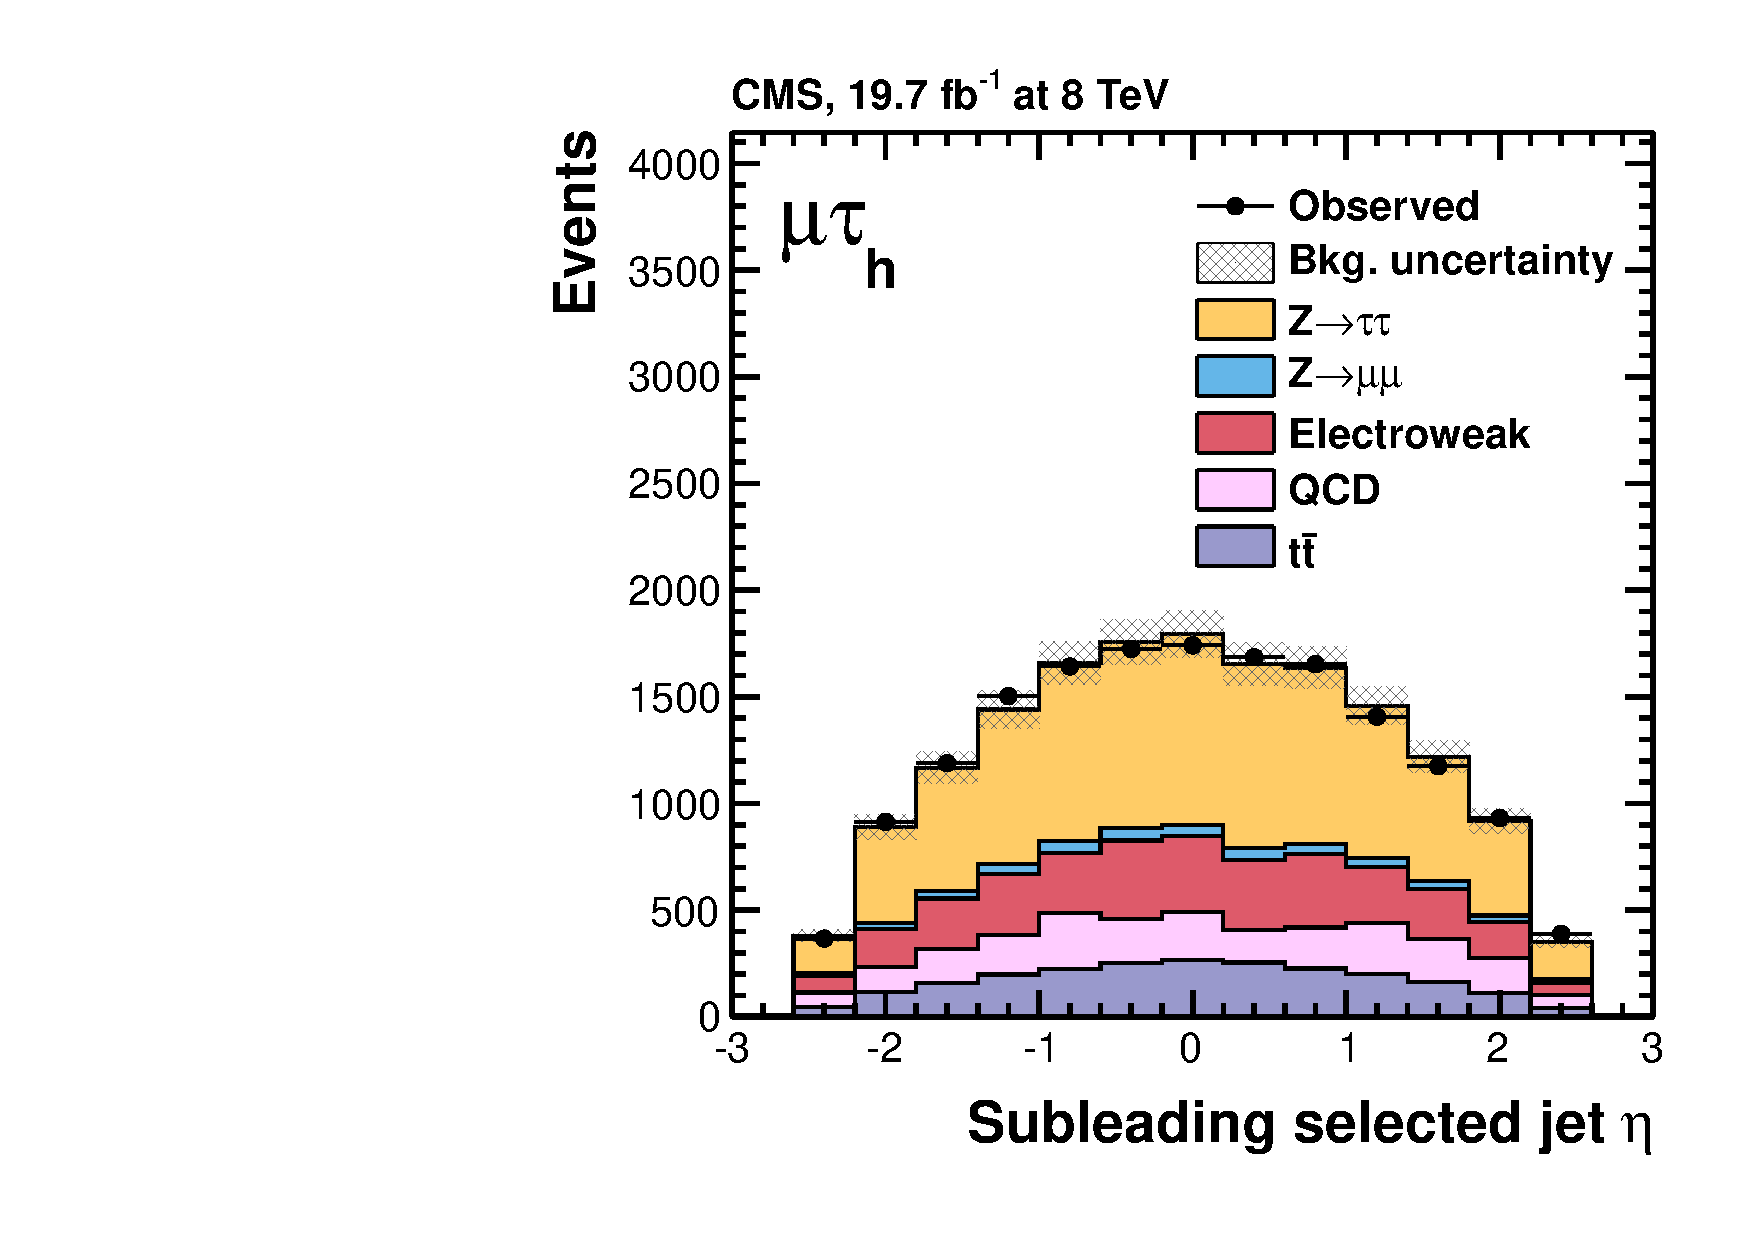
\includegraphics[width=0.4\textwidth]
      {plots/Hhh/ControlPlots/mutau/prebjeteta_2_2jetinclusive_mt_2012.pdf}} 

\subfloat[]{
    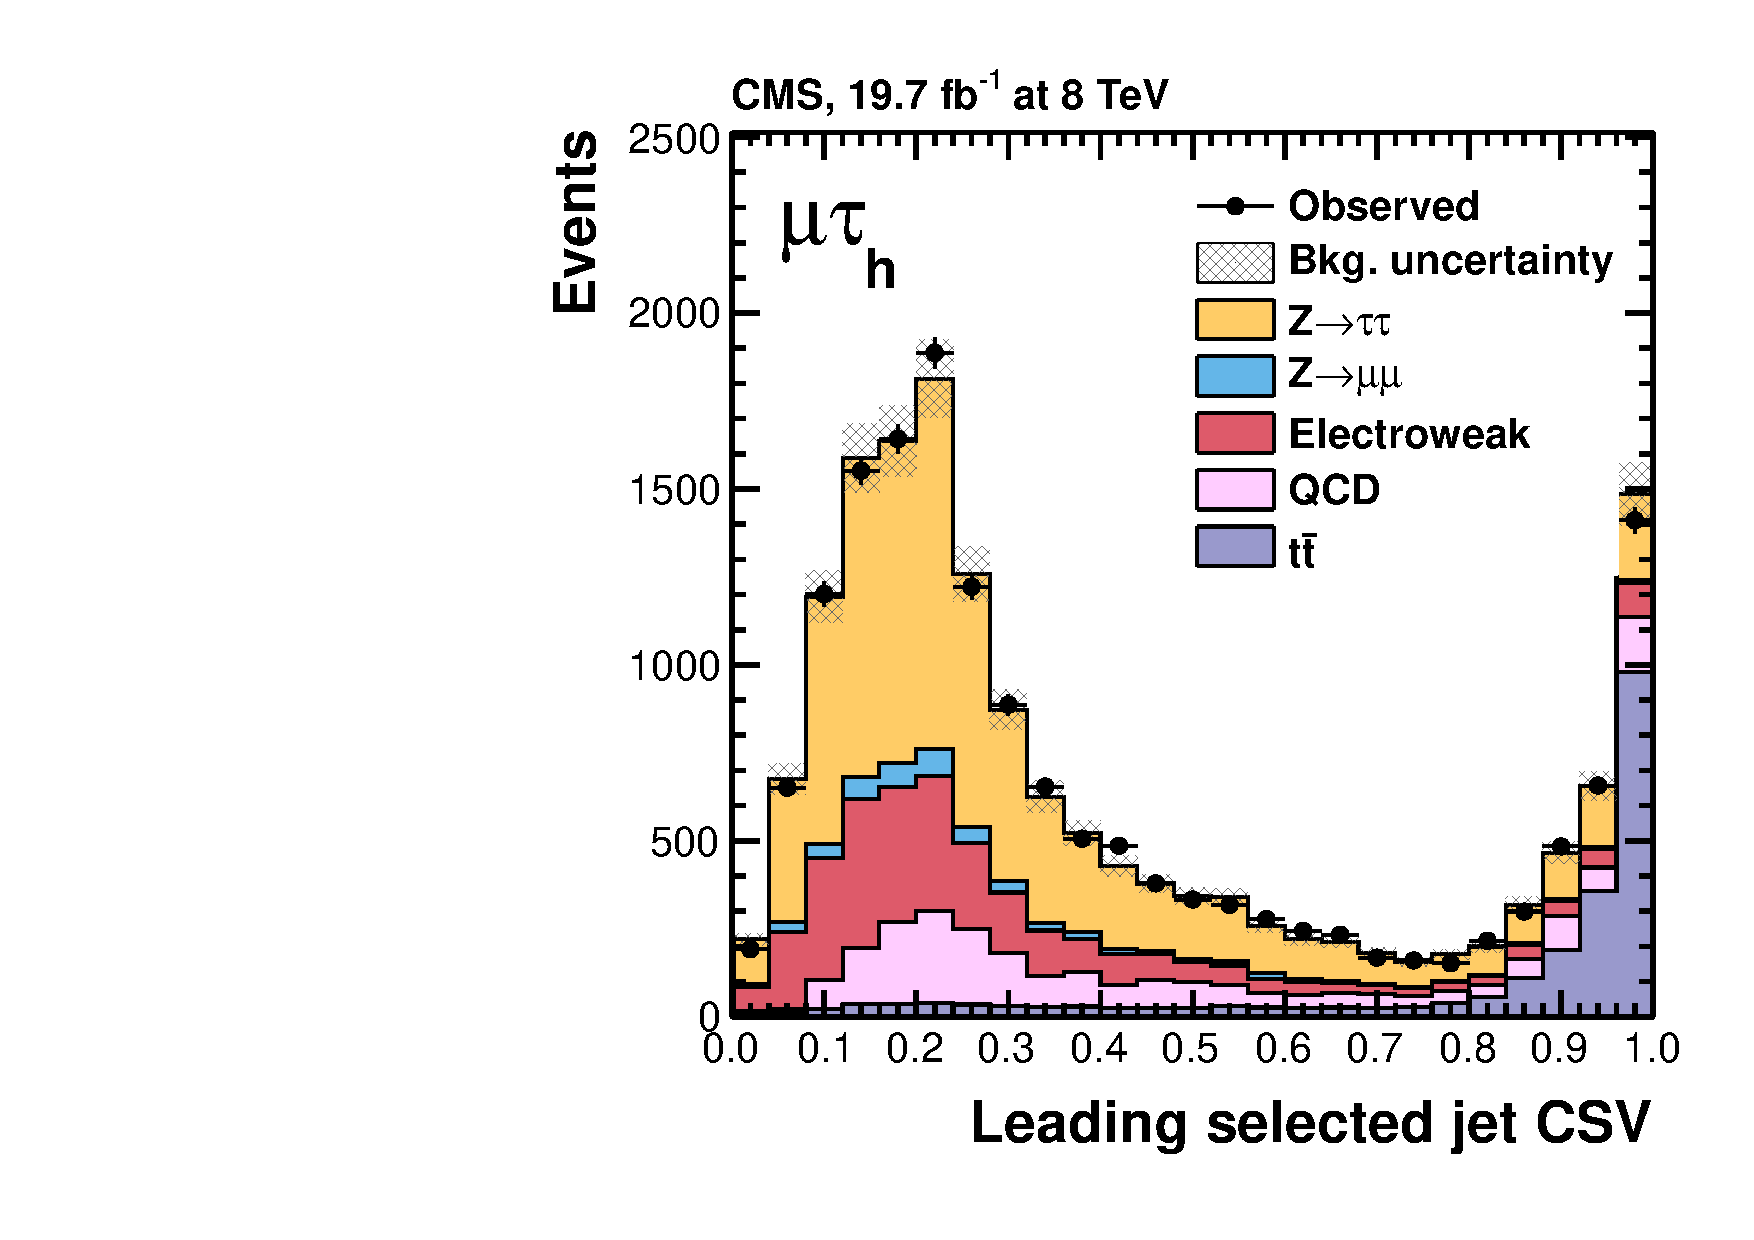
\includegraphics[width=0.4\textwidth]
      {plots/Hhh/ControlPlots/mutau/prebjetbcsv_1_2jetinclusive_mt_2012.pdf}}
\subfloat[]{
    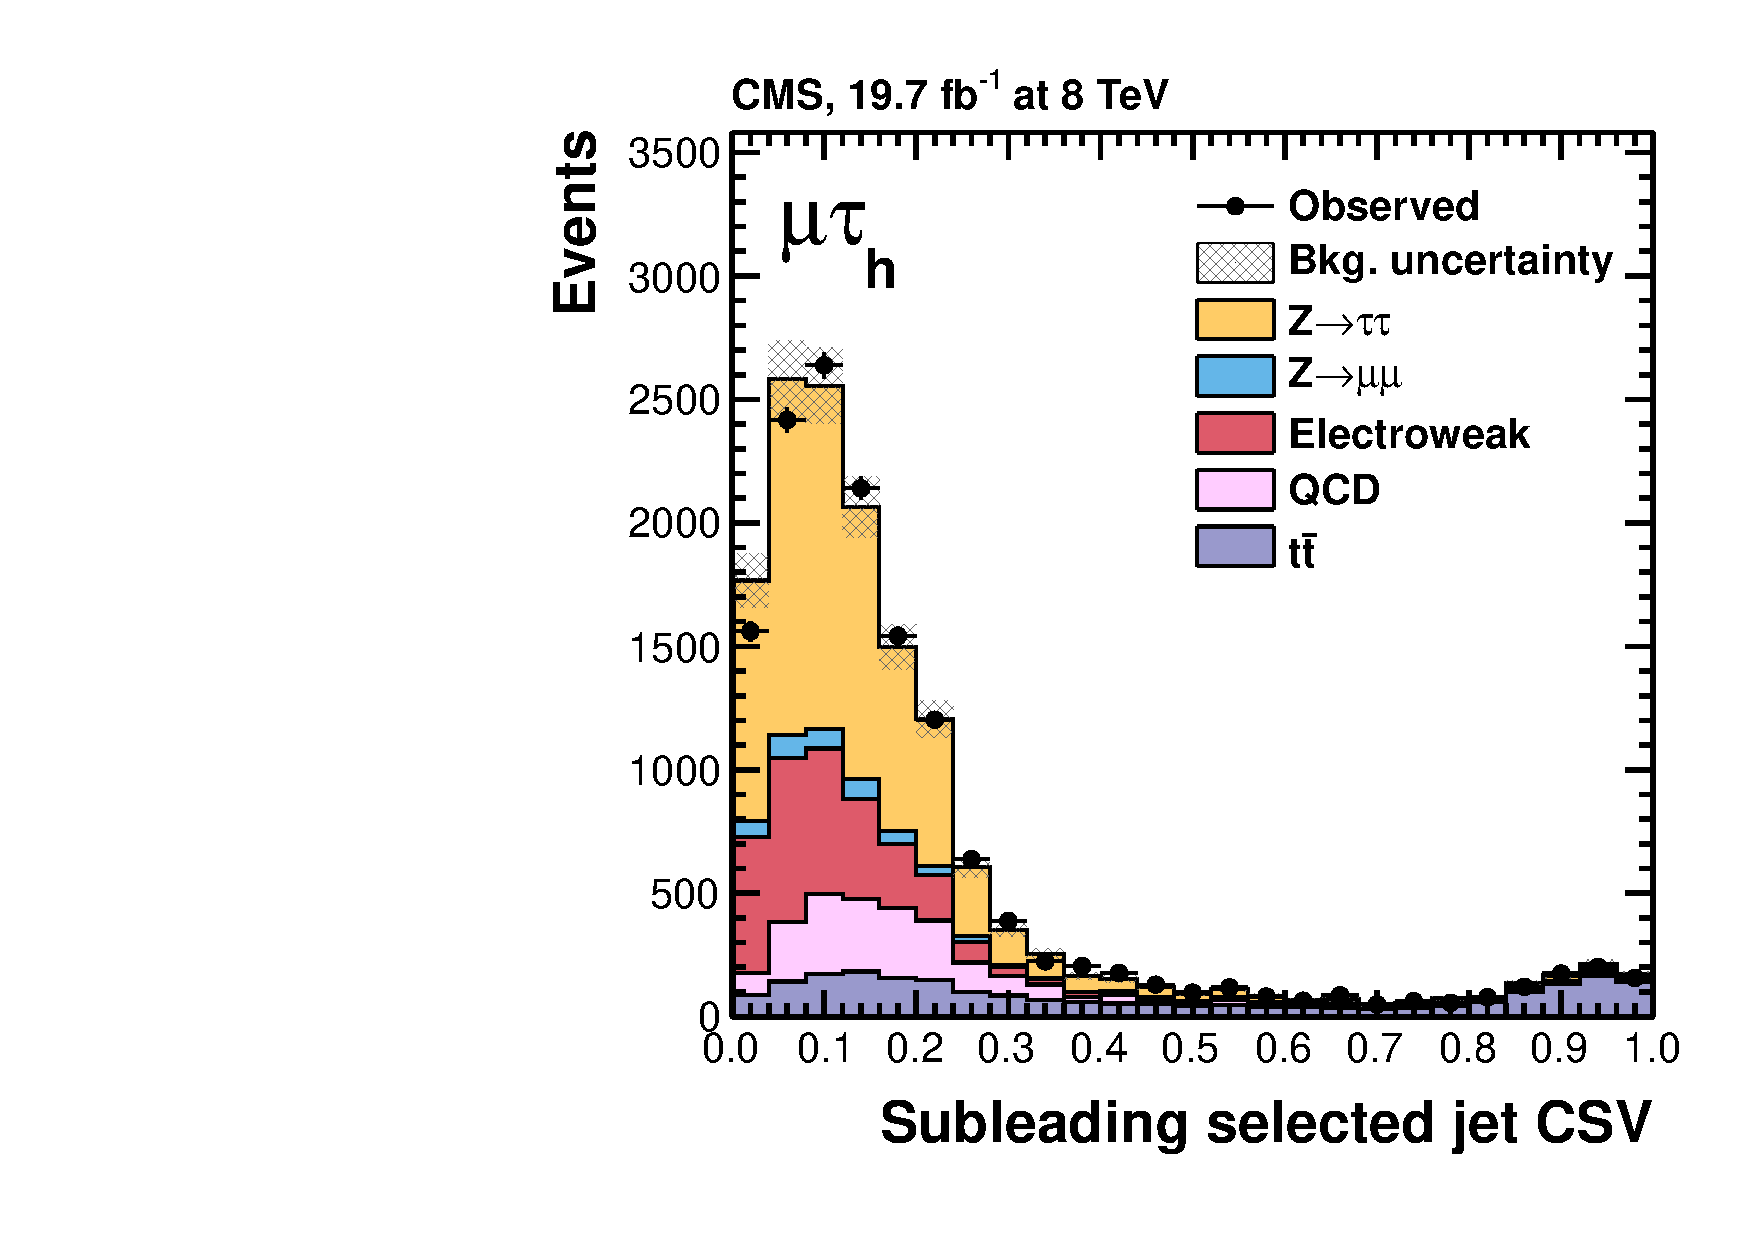
\includegraphics[width=0.4\textwidth]
      {plots/Hhh/ControlPlots/mutau/prebjetbcsv_2_2jetinclusive_mt_2012.pdf}}
\end{center}
\caption{
  Distributions of relevant kinematic variables related to the b-jet candidates for
  events with at least 2 jets in the $\mu\tau_{had}$ channel. The plots/Hhh show the
  $\pt$ (top), $\eta$ (centre) and CSV discriminator (bottom) for the leading
  jet (left) and sub-leading jet (right). Here leading and sub-leading refers to
  the jet with the highest and second highest CSV value respectively.
  Expected background contributions are shown for the values of nuisance parameters
  obtained by fitting the signal plus background hypothesis to the data.
}
\label{fig:resultsControlPlotsJetPairMuTau}
\end{figure} 

\begin{figure}
\setlength{\unitlength}{1mm}
\begin{center}
\begin{picture}(150,210)(0,0)
\put(-5.5, 140.0){\mbox{\includegraphics*[height=68mm]
  {plots/Hhh/ControlPlots/etau/mt_1_2jetinclusive_et_2012.pdf}}}
\put(78.0, 140.0){\mbox{\includegraphics*[height=68mm]
  {plots/Hhh/ControlPlots/etau/met_2jetinclusive_et_2012.pdf}}}
\put(-5.5, 70.0){\mbox{\includegraphics*[height=68mm]
  {plots/Hhh/ControlPlots/etau/pt_1_2jetinclusive_et_2012.pdf}}}
\put(78.0, 70.0){\mbox{\includegraphics*[height=68mm]
  {plots/Hhh/ControlPlots/etau/pt_2_2jetinclusive_et_2012.pdf}}}
\put(-5.5, 0.0){\mbox{\includegraphics*[height=68mm]
  {plots/Hhh/ControlPlots/etau/eta_1_2jetinclusive_et_2012.pdf}}}
\put(78.0, 0.0){\mbox{\includegraphics*[height=68mm]
  {plots/Hhh/ControlPlots/etau/eta_2_2jetinclusive_et_2012.pdf}}}
\end{picture}
\end{center}
\caption{
  Distributions of relevant kinematic variables for events with at least 2 jets
  in the $e\tau_{had}$ channel. The variable $m_{T}$ is shown in the top left
  plot and a cut of $m_{T} < 30$ is applied for the rest of the plots/Hhh, which
  show the $\MET$ (top right) $\pt$ of the electron (left centre) and tau (right
  centre), and $\eta$ of the electron (left bottom) and tau (right bottom).
  Expected background contributions are shown for the values of nuisance parameters
  obtained by fitting the signal plus background hypothesis to the data.
}
\label{fig:resultsControlPlotsTauPairETau}
\end{figure} 

\begin{figure}
\setlength{\unitlength}{1mm}
\begin{center}
\begin{picture}(150,210)(0,0)
\put(-5.5, 140.0){\mbox{\includegraphics*[height=68mm]
  {plots/Hhh/ControlPlots/etau/prebjetpt_1_2jetinclusive_et_2012.pdf}}}
\put(78.0, 140.0){\mbox{\includegraphics*[height=68mm]
  {plots/Hhh/ControlPlots/etau/prebjetpt_2_2jetinclusive_et_2012.pdf}}}
\put(-5.5, 70.0){\mbox{\includegraphics*[height=68mm]
  {plots/Hhh/ControlPlots/etau/prebjeteta_1_2jetinclusive_et_2012.pdf}}}
\put(78.0, 70.0){\mbox{\includegraphics*[height=68mm]
  {plots/Hhh/ControlPlots/etau/prebjeteta_2_2jetinclusive_et_2012.pdf}}}
\put(-5.5, 0.0){\mbox{\includegraphics*[height=68mm]
  {plots/Hhh/ControlPlots/etau/prebjetbcsv_1_2jetinclusive_et_2012.pdf}}}
\put(78.0, 0.0){\mbox{\includegraphics*[height=68mm]
  {plots/Hhh/ControlPlots/etau/prebjetbcsv_2_2jetinclusive_et_2012.pdf}}}
\end{picture}
\end{center}
\caption{
  Distributions of relevant kinematic variables related to the b-jet candidates for
  events with at least 2 jets in the $e\tau_{had}$ channel. The plots/Hhh show the
  $\pt$ (top), $\eta$ (centre) and CSV discriminator (bottom) for the leading
  jet (left) and sub-leading jet (right). Here leading and sub-leading refers to
  the jet with the highest and second highest CSV value respectively.
  Expected background contributions are shown for the values of nuisance parameters
  obtained by fitting the signal plus background hypothesis to the data.
}
\label{fig:resultsControlPlotsJetPairETau}
\end{figure} 





